\[	
	u(x_0, y_0, z_0) = \iint\limits_S \left(u \derp{G}{n}{} - G \derp{u}{n}{} \right)\, dS + \iiint\limits_\Omega F \, d\Omega = \begin{cases}
		2 \pi u &A \in \Omega\\
		\pi u & A \in S\\
		0 &  A\notin \Omega\\
	\end{cases}
\]
где $F(x, y, z) = \Delta u$.\\

В плоском случае фундаментальным решением задачи Лапласа является $\ln \frac{1}{r}$.
Рассмотрим задачу.
\[
	\Delta u = 0
\]
\[
	\derp{u}{x}{2} + \derp{u}{y}{2} = 0
\]
\[
	r= \sqrt{(x - x_0)^2 + (y - y_0)^2}
\]
\[
	u = \ln \frac{1}{r} = - \ln r
\]
\begin{align*}
	&\derp{u}{x}{} = - \frac{1}{r} \cdot \derp{r}{x}{} = - \frac{1}{r^2 (x - x_0)}\\
	&\derp{u}{x}{2} = - \frac{1}{r^2} + \frac{2  (y - y_0)^2}{r^4}\\
	&\derp{u}{x}{2} + \derp{u}{y}{2} = -\frac{2}{r^2} + \frac{2 \left[ (x - x_0)^2 + (y - y_0)^2 \right]}{r^4} = - \frac{2}{r^2} + \frac{2}{r^2} = 0
\end{align*}
\[	
	\Delta G = 0
\]
\[
	G\big|_\Gamma = 0
\]
\[
	G = W - \ln \frac{1}{r_AP} 
\]
\[
	\oint\limits_\Gamma \left(u \derp{v}{n}{} - v \derp{u}{n}{} \right)\, d \gamma = \iint\limits_S \left(u \Delta - v \Delta u \right)\, dS
\]
Радиус окружности $\Gamma_1 = \varepsilon$.
\begin{figure}[h!]
	\centering
	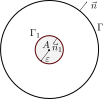
\includegraphics{figGreenMethTwoDim.pdf}
\end{figure}
\[
	\oint\limits_\Gamma \left(u \derp{v}{n}{} - v \derp{u}{n}{} \right)\, d\gamma + \oint\limits_{\Gamma_1} \left(u \derp{v}{n_1}{} - v \derp{u}{n_1}{} \right)\, d\gamma = 0
\]
\[
	v = G
\]
Нас интересует интеграл вида
\[
	\oint\limits_{\Gamma_1} \left(u \derp{G}{n_1}{} - G \derp{u}{n_1}{} \right)\, d\gamma
\]
Если интеграл берётся по окружности радиуса $\varepsilon$, то:
\[
	\derp{}{n_1}{} = - \derp{}{r}{}, \qquad dr = \varepsilon\, d\theta
\]
\[
	\iint\limits_0^{2\pi} \left( - u \derp{G}{r}{} + G \derp{u}{r}{} \right) \varepsilon d\theta = \int\limits_0^{2\pi} \left(- u \derp{w}{r}{} + w \derp{u}{r}{} + u \derp{}{r}{} \left(\ln \frac{1}{r} \right) - \ln \frac{1}{r} \derp{u}{r}{}\right) \cdot \varepsilon
\]
\[
	(- \ln r )' = - \frac{1}{r}
\]
Перейдём к пределу:
\[
	\lim\limits_{\varepsilon \to 0} \oint\limits_{\Gamma_1} \left(u \derp{G}{n_1}{} - G \derp{u}{n_1}{} \right) = \\ 
	=	\lim\limits_{\varepsilon \to 0} \int\limits_0^{2 \pi} \left(- u \derp{w}{r}{} + w \derp{u}{r}{} \right)\, d\theta - \lim\limits_{\varepsilon \to 0} \varepsilon \int\limits_0^{2 \pi} \left[u \frac{1}{\varepsilon}  + \derp{u}{r}{} \ln \varepsilon\right]\, d\theta  
\]
Так как $u, w$ --- непрерывно гладкие функции, то
\[
	\varepsilon \ln \varepsilon \underset{\varepsilon \to 0}{\to} 0
\]

В итоге получаем 
\[
	- \int\limits_0^{2 \pi} u \, d \theta
\]
Значит:
\[
	\oint\limits_\Gamma \left(u \derp{v}{n}{} - v \derp{u}{n}{} \right)\, d\gamma - \underbrace{\int\limits_0^{2 \pi} u\, d \theta}_{u(x_0, y_0) 2 \pi} = 0
\]
так как интегрируем в малой области.
